\documentclass{article}

\usepackage{times}
\usepackage{graphicx}
\usepackage{amsmath}
\usepackage{amsfonts}
\usepackage{subfigure}
\usepackage{natbib}
\usepackage{algorithm}
\usepackage{algorithmic}
\usepackage{lipsum}
\usepackage{todonotes}
\usepackage[accepted]{icml2017}
\icmltitlerunning{CS 287 Final Project Template}

\newcommand{\eval}[2]{\Big|_{#1}^{#2}}
\newcommand{\vect}[1]{\boldsymbol{#1}}
\newcommand{\R}{\mathbb{R}}
\newcommand{\E}{\mathbb{E}}
\newcommand{\norm}[1]{\left\lVert#1\right\rVert}

\usepackage{hyperref}
\usepackage{booktabs} % Top and bottom rules for tables
\newcommand{\given}{\,\vert\,}


\begin{document}

\twocolumn[
\icmltitle{Style Transfer with Disentangled ARAEs}
\begin{icmlauthorlist}
  \icmlauthor{Alex Lin}{}
\icmlauthor{Melissa Yu}{}
\end{icmlauthorlist}

\vskip 0.3in
]

\begin{abstract}
In this project, we examine the \emph{style transfer} problem, which asks us to change one attribute of a sentence (e.g. sentiment) without altering the overall style and grammar of that sentence.  Our approach involves the Adversarially Regularized Autoencoder (ARAE) \cite{arae} to explicitly disentangle the latent attribute of interest from the other stylistic attributes that we wish to keep.  We compare the performance of this Disentangled ARAE to results from the original ARAE on the Yelp dataset.
\end{abstract}

\section{Introduction}
\label{sec:introduction}

This project explores the \emph{style transfer} problem.  Given a source sentence and some attribute of that sentence (e.g. sentiment, formality, time period), we wish to produce another sentence that has the same overall style and grammar of the original sentence, yet differs in its attribute of interest.  For example, if the attribute of interest is formality, here might be an example of style transfer \cite{rao}:

\begin{center}
Informal: \emph{I'd say it is punk though.} \\
Formal: \emph{However, I do believe it to be punk.}
\end{center}

The first sentence is informal, yet this lack of formality is stripped away in the second sentence, which holds the same structure and meaning.  Here is another example with Shakespearean English vs. Modern English.

\begin{center}
Shakespearean English: \emph{So thrive my soul --} \\
Modern English: \emph{My soul depends on it --}
\end{center} 

Having a model that can freely switch and translate between these modes can be quite useful.  There have been models proposed that tackle this exact problem in natural language processing, such as the Adversarially Regularized Autoencoder (ARAE) \cite{arae}.  In this work, we change some aspects of this model to formulate the Disentangled ARAE for the style transfer problem.  Section 2 covers some background and Section 3 presents related work on the problem.  Section 4 formally presents the mathematical model and Section 5 covers the training procedure.  Section 6 covers methods, and Section 7 covers results and a discussion.  

\section{Background}
While latent variable models have enjoyed success in tackling computer vision problems, they have generally been less effective in the domain of natural language processing (NLP).  One particularly useful application of latent variable models to NLP is the \emph{style transfer} problem, in which we seek to transfer the content
of a source sentence to a new sentence that follows certain presentation constraints specified by the user. Specifically, in this paper we consider the problem of sentiment transfer, in which we seek to preserve the content and style of a sentence but modify its sentiment from positive to negative, or vice versa.

The problem of \emph{unaligned style transfer} seeks to perform style transfer without using parallel data (like that typically used for sentence translation or summarization), but instead, simply training on a non-parallel corpus of sentences which cover the same content distributions, but are not explicitly paired.


\section{Related Work}

\subsubsection{Generative Adversarial Networks} \label{sssec:gan}
The generative adversarial network (GAN) \cite{gan} framework establishes a min-max game between two neural networks, the generator $G$ and the discriminator $D$, in order to match the generative process to the data distribution. Suppose the generator network $G(\vect{z})$ maps some hidden representation $\vect{z}$ to the data space, and the discriminator network $D(\vect{x})$ predicts the probability that a sample $\vect{x}$ comes from the true data distribution $p_d$ (positive samples), and not $G$'s generative process (negative samples). The objective is
\begin{equation}
\min_G \max_D \ \E_{p_d(\vect{x})} [\log D(\vect{x})] + \E_{p(\vect{z})} [\log (1 - D(G(\vect{z})))]
\end{equation}
The network consists of the discriminator, which achieves the best classification accuracy over samples of $\vect{x}$, and the generator, which maximally confuses this best discriminator, so that $D(\vect{x}) = 1/2$.

\subsubsection{Semi-Supervised Adversarial Autoencoders} \label{sssec:aae}

Adversarial autoencoders (AAE) \cite{aae} are probabilistic autoencoders which perform variational inference by utilizing generative adversarial networks to regularize the encoder. Let $\vect{x}$ be the input following the true data distribution $p_d(\vect{x})$, and let $\vect{z}$ be the latent code vector generated by the autoencoder. We wish to approximate the encoding distribution $q(\vect{z}\given\vect{x})$, informed by the prior $p(\vect{z})$. Additionally, we would also like to estimate the decoding distribution $p(\vect{x}\given\vect{z})$. 

Recall the variational autoencoder's objective \cite{vae}
\begin{equation}
\min_q \
\E_{q(\vect{z}\given\vect{x})} [-\log p(\vect{x}\given\vect{z})] + KL(q(\vect{z}\given\vect{x}) \ \vert\vert \ p(\vect{z}))
\end{equation}
AAE simply replaces the KL divergence term with an adversarial network on top of the latent code, which guides the aggregated posterior
\begin{equation}
q(\vect{z}) = \int_{\vect{x}} q(\vect{z}\given\vect{x}) p_d(\vect{x}) d\vect{x}
\end{equation}
to match the prior $p(\vect{z})$. In this model, the encoder of the autoencoder is also the generator of the adversarial network: $G(\vect{z}) = q(\vect{z}\given\vect{x})$. The model has two objectives; the first seeks to minimize the reconstruction error $\mathcal{L}(\vect{x}, \vect{x}')$ of the network, while the second GAN objective seeks to match the generative process for $\vect{z}$ with the prior process. 

Semi-supervised AAE leverages the generative description of unlabeled data to achieve better classification performance than can be obtained using only labeled data. In this scheme, data $\vect{x}$ is generated from a combination of a latent class vector $\vect{y} \sim p_y(\vect{y})$ and a latent ``style'' vector $\vect{z} \sim p_z(\vect{z})$. The encoder is thus $q(\vect{y}, \vect{z} \given \vect{y})$ and the decoder is $p(\vect{x} \given \vect{y}, \vect{z})$. Adversarial networks $D_y(\vect{y})$ and $D_z(\vect{z})$ are attached on top of both latent codes to enforce the two prior distributions.


\section{Model} 

The basic ARAE architecture follows adversarial autoencoders (AAEs) in combining variational autoencoders (VAEs) with GANs (generative adversarial networks) \cite{arae}.  A diagram of how this model can be used for unaligned style transfer can be found in Figure 1.

Given a vocabulary $\mathcal{V}$, each input to the ARAE is a sentence $\vect{x} = \{x_1, x_2, \ldots\}$ where each word $x_t \in \mathcal{V}$.  We define $\mathcal{X} = \mathcal{V}^T$ (where $T$ is the variable length of a sentence) as the observation space and $\mathcal{C}$ as the latent code space.  In the VAE part of the ARAE, $\vect{x}$ is passed through an encoder $q_\phi : \mathcal{X} \to \mathcal{C}$ to form a latent code $\vect{c} = q_\phi(\vect{x})$.  This code represents the stylistic attributes of the sentence.  

In the style transfer problem, we assume that $\vect{x}$ has some true attribute/class of interest $y^* \in \mathcal{Y}$.  We wish to generate some $\tilde{\vect{x}}$ that has a different attribute/class $\tilde{y} \neq y^*$ such that its corresponding stylistic attributes except for $\tilde{y}$ are the same as those of $\vect{x}$.

Note that $q$ is represented in our architecture as a neural network with parameters $\phi$.

The latent code is then put through a classifier $f_u : \mathcal{C} \to [0, 1]$ that returns the probability of the sentence having the attribute of interest.  (Note that in this case, we assume that the attribute is binary -- e.g. positive or negative sentiment).  Similarly, $f$ is also a neural network with parameters $u$.  

Let the decision of the classifier be $y \in \{0, 1\}$, where 1 corresponds to one class and 0 correspond to the other.  During classification training, this decision is compared to the true label $y^* \in \{0, 1\}$.  This classifier is in the ARAE architecture so that we can use the encoder to adversarially train against it, thereby ensuring that $\vect{c}$ does not hold any information about $y^*$ -- a property that is necessary for the style transfer procedure.  

Then, conditioning on the latent code $\vect{c}$ and the true class $y^*$, the decoder $r_\psi : \mathcal{C} \times \{0, 1\} \to \mathcal{X}$ returns a reconstructed sentence $\vect{x}' = r_\psi(\vect{c}, y^*)$.  Note that if we wanted to transfer the style of the sentence to a sentence in the other class, we could simply decode with $r_\psi(\vect{c}, 1 - y^*)$.  Again, $r$ is a neural network (or a series of neural networks) with parameters $\psi$.  See Section 5 for additional details.      

The latent code $\vect{c}$ is adversarially regularized by a GAN so that its distribution does not deviate too far from a flexible prior.  The base distribution of the GAN is $\mathcal{N}(\vect{0}, \vect{I})$ where $\vect{I}$ is the identity matrix.  A generator $g_\theta : \mathbb{R}^{\text{dim}(\vect{I})} \to \mathcal{C}$ takes samples $\vect{v} \sim \mathcal{N}(\vect{0}, \vect{I})$ and tries to fool a corresponding discriminator $d_w : \mathcal{C} \to [0, 1]$ by using fake codes $\vect{c}' = g_\theta(\vect{v})$.  Both the generator $g$ and the discriminator $d$ are neural networks with parameters $\theta$ and $w$ respectively.

The Disentangled ARAE, our proposed modification to this model, aims to explicitly separate the attribute of interest $y^*$ from the style of the sentence.  Here, "style" refers to all latent variables except for $y^*$.  The motivation is that working with this structure allows us to not have to adversarially train the classifier, which could be unstable and also increase the computational time of training the model.  Our inspiration comes from the completely disentangled structure of the original Adversarial Autoencoder that was used for supervised and semi-supervised training \cite{aae}.

The main change that we make is to have the latent code $\vect{c}$ be passed through a multilayer perceptron $a_\alpha : \mathcal{C} \to \mathcal{Z}$  where $\alpha$ is the parameters of the network and $\mathcal{Z}$ is the latent style space.  The result is the latent style $\vect{z} \in \mathcal{Z}$.  Separately, $\vect{c}$ is also passed through the classifier $f_u$ to generate $y$ from $f_u(\vect{c})$.  Thus, we have disentangled the style from the class.  

The style $\vect{z}$ (not the code $\vect{c}$) will now be passed along with the class $y$ to the decoder, redefined as $r_\psi : \mathcal{Z} \times \{0, 1\} \to \mathcal{X}$.  In addition, the generator $g_\theta : \mathbb{R}^{\text{dim}(\vect{I})} \to \mathcal{Z}$ of the Disentangled ARAE is used to regularize $\vect{z}$ instead of $\vect{c}$.  See Figure 1 for the architecture of the model.       

            
\begin{figure}
  \centering
  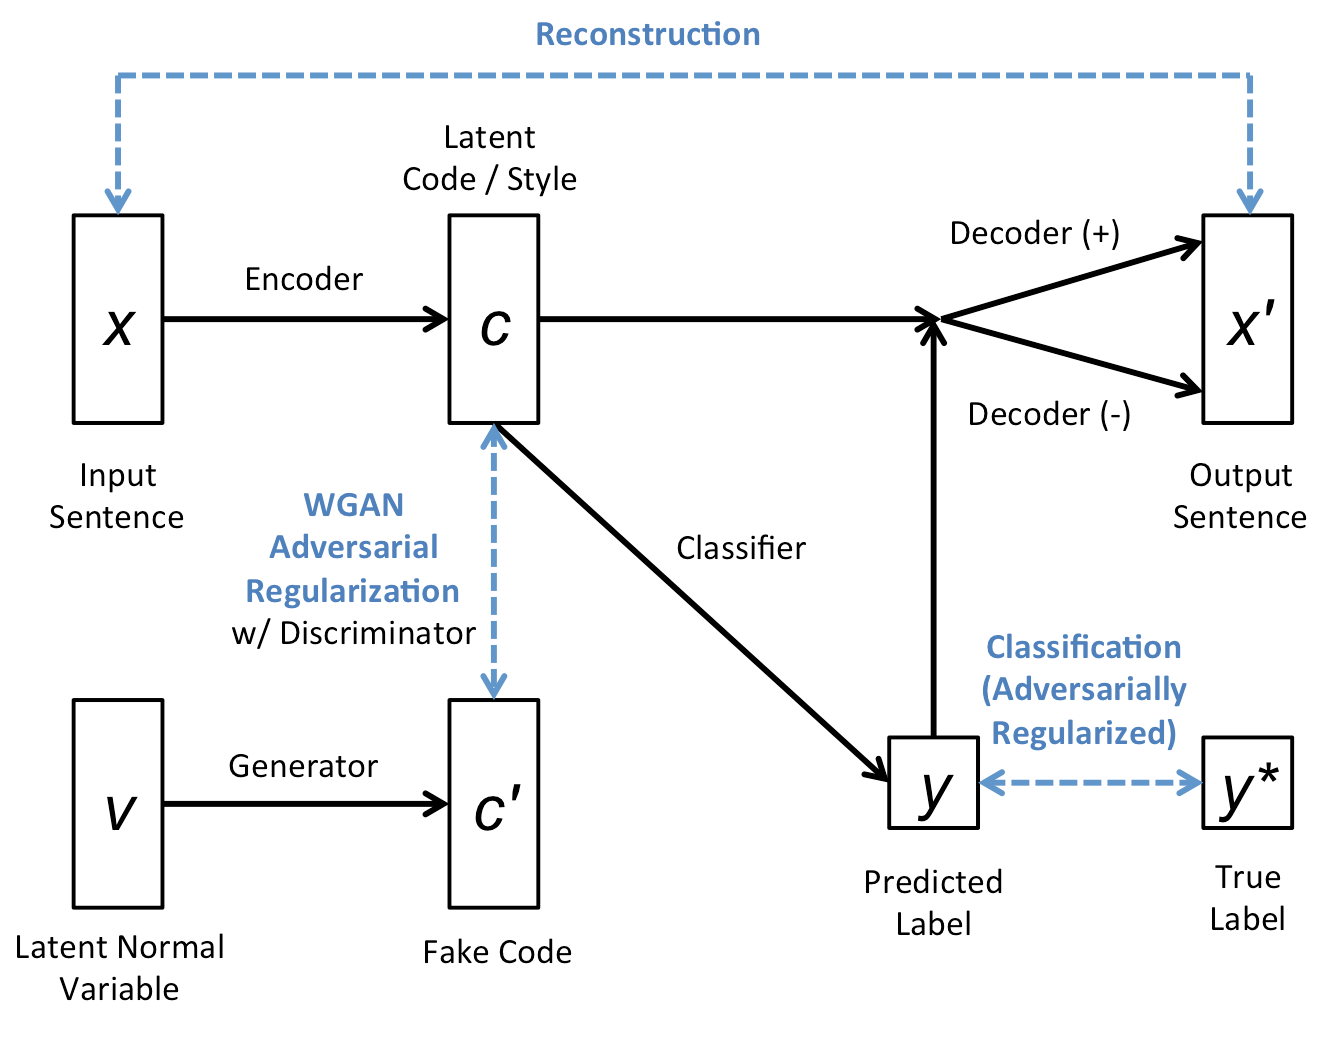
\includegraphics[scale=0.15]{img/arae}
  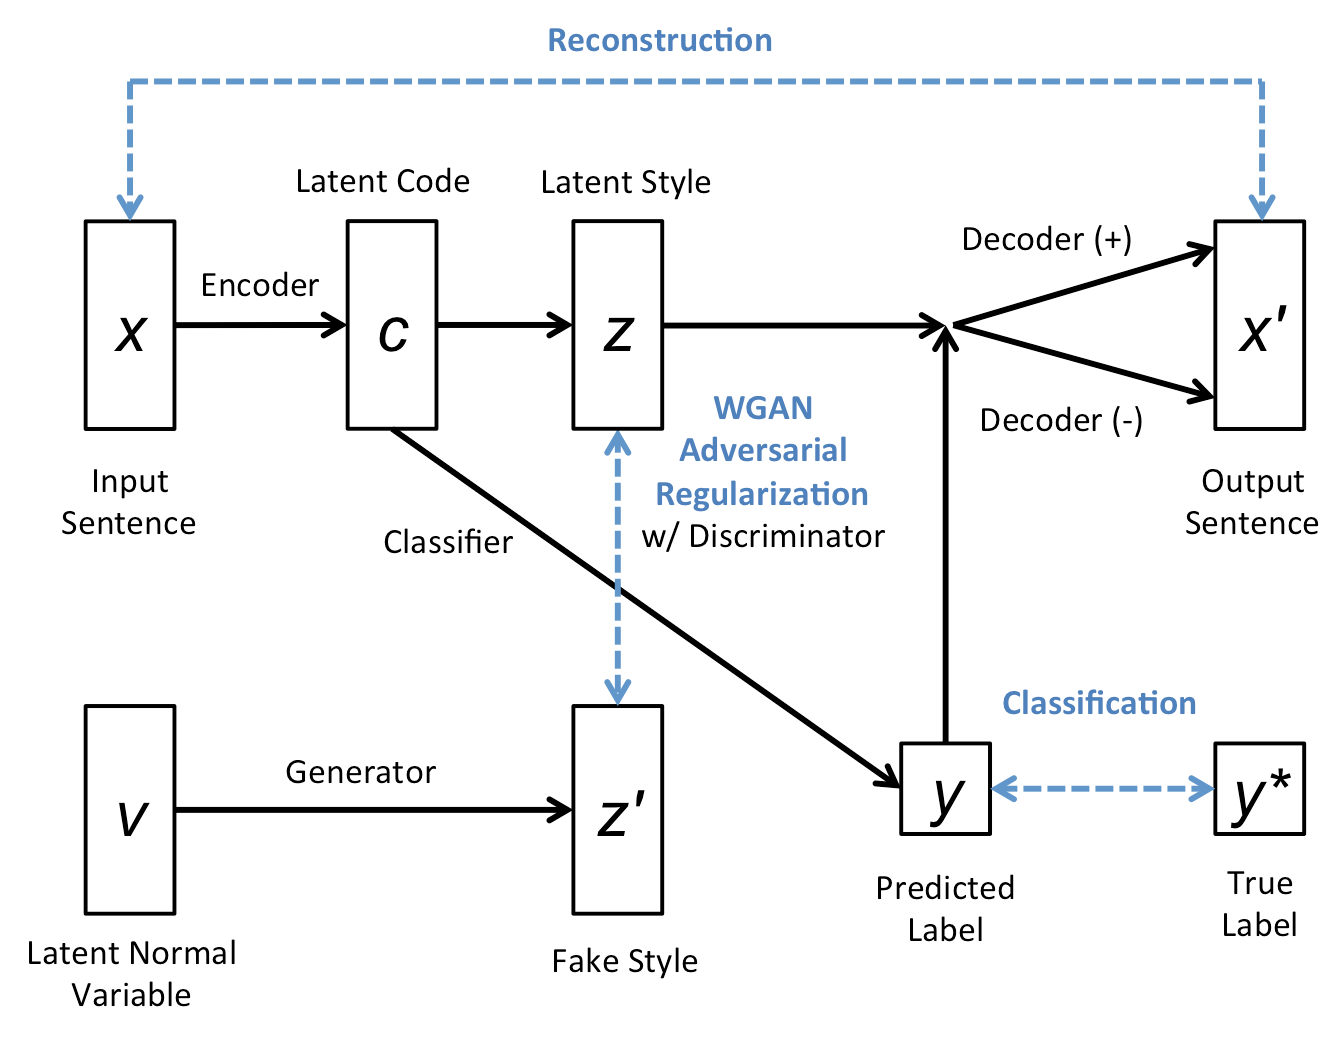
\includegraphics[scale=0.15]{img/disentangled-arae}
  \caption{\label{fig:diagram} Diagrams and training procedures for ARAE (\emph{top}) and our modified Disentangled ARAE (\emph{bottom}).}
\end{figure}


\section{Training}

The ARAE trains its various components in several different steps so that it can construct a desirable latent code space $\mathcal{C}$.  First, the ARAE trains the reconstruction loss of the autoencoder.  This loss is defined as the cross-entropy between the data's true distribution and the model's assigned distribution 
\begin{align*}
\mathcal{L}_\text{rec}(\vect{x}) &=  y^* \cdot \log r_\psi(q_\phi(\vect{x}), y^*)  \\
&+ (1 - y^*) \cdot  \log \left[1 - r_\psi(q_\phi(\vect{x}), y^*) \right]
\end{align*} 
Note in Figure 1 that there are two decoders in style transfer -- one for the positive class $r_\psi^1: \mathcal{C} \to \mathcal{X}$ and one for the negative class $r_\psi^0 : \mathcal{C} \to \mathcal{X}$.  In fact, during training, we choose the decoder to use for $\vect{x}$ based on the true class $y^*$.  That is, 
\begin{align*}
r_\psi(\vect{c}, y^*) = r_\psi^{y^*}(\vect{c})
\end{align*}    
During reconstruction training, we backpropagate the gradients of $\mathcal{L}_\text{rec}$ to update the encoder's parameters $\phi$ and the decoder's parameters $\psi$.  

Second, the ARAE trains the discriminator to minimize its loss function.
Given a true latent code $\vect{c}$, this is 
\begin{align*}
\mathcal{L}_\text{disc}^\text{true}(\vect{c}) = \log d_w(\vect{c})
\end{align*}
whereas if given a generated latent code $\vect{c'}$ this is
\begin{align*}
\mathcal{L}_\text{disc}^\text{fake}(\vect{c}') = \log \left[1 - d_w(\vect{c}')\right]
\end{align*}
The discriminator's parameters $w$ are then updated during backpropagation and also contained within the ball $[-\epsilon, \epsilon]^{\text{dim}(w)}$ for some hyperparameter $\epsilon$.  

Third, the ARAE trains the classifier to minimize its loss function.
\begin{align*}
\mathcal{L}_\text{class}(\vect{c}, y^*) = y^* \cdot \log f_u(\vect{c}) + (1 - y^*) \cdot \log [1 -  f_u(\vect{c})]
\end{align*} 
The classifier's parameters $u$ are then updated during backpropagation.  

Fourth, the ARAE trains the encoder adversarially to maximize the classifier's loss function and minimize  
\begin{align*}
-\mathcal{L}_\text{class}(q_\phi(\vect{x}), y^*)
\end{align*}
The encoder's parameters $\phi$ are then updated during backpropagation.

And finally, the ARAE trains both the encoder and the generator adversarially to maximize the discriminator's loss function.  The encoder wishes to minimize 
\begin{align*}
-\mathcal{L}_\text{disc}^\text{true}(q_\phi(\vect{x}))
\end{align*}
whereas the generator wishes to minimize
\begin{align*}
-\mathcal{L}_\text{disc}^\text{fake}(g_\theta(\vect{v}))
\end{align*}
where $\vect{v} \sim \mathcal{N}(\vect{0}, \vect{I})$.  Again, we do backpropagation on these losses to update $\phi$ for the encoder and $\theta$ for the generator.  The full algorithm for ARAE is given in Algorithm 1.

Disentangled ARAE is slightly different from the original ARAE setup.  First, Disentangled ARAE also trains reconstruction, but has an intermediate MLP converting $\vect{c}$ to $\vect{z}$.  That is,
\begin{align*}
\mathcal{L}_\text{rec}(\vect{x}) &=  y^* \cdot \log r_\psi(a_\alpha((q_\phi(\vect{x})), y^*)  \\
&+ (1 - y^*) \cdot  \log \left[1 - r_\psi(a_\alpha(q_\phi(\vect{x})), y^*) \right]
\end{align*} 

Again, there are two decoders -- one for each class.  However, they map $\mathcal{Z}$ to $\mathcal{X}$ instead.  In addition, when we backpropagate the gradients, we are tuning $\alpha$ for $a$ in addition to the parameters of the encoder and the decoder.  

Second, the discriminator's loss in Disentangled ARAE is defined on the latent style $\vect{z}$ instead of the latent code $\vect{c}$.

Third, the classifier in Disentangled ARAE minimizes its loss function in the same way as before. However, there is no adversarial training of the encoder, because part of the objective of the project was to investigate the necessity of this step for the style transfer problem.  

Finally, both the encoder and the generator are trained adversarially, yet there is an MLP in between the discriminator and the encoder.  That is, the encoder wishes to minimize
\begin{align*}
-\mathcal{L}_\text{disc}^\text{true}(a_\alpha(q_\phi(\vect{x})))
\end{align*}
whereas the generator wishes to minimize
\begin{align*}
-\mathcal{L}_\text{disc}^\text{fake}(g_\theta(\vect{v}))
\end{align*}   

The full details for Disentangled ARAE are in Algorithm 2.

\begin{algorithm}
  \begin{algorithmic}
    \FOR{each training iteration}{
    	\STATE{\textbf{(1) Train Reconstruction}}
	\STATE{Sample $(\vect{x}^{(1)}, y^{*(1)}), \ldots, (\vect{x}^{(M)}, y^{*(M)})$ from data.}
	\STATE{Backprop loss $\frac{1}{M} \sum_{m=1}^{M} \mathcal{L}_{\text{rec}}(\vect{x}^{(m)})$ to update $\phi, \psi$.}
	\STATE{\textbf{(2) Train Discriminator}}
	\STATE{Sample $(\vect{x}^{(1)}, y^{*(1)}), \ldots, (\vect{x}^{(M)}, y^{*(M)})$ from data.}
	\STATE{Compute $\vect{c}^{(m)} = q_\phi(\vect{x}^{(m)})$ for $m = 1, \ldots, M$.}
	\STATE{Sample $\vect{v}^{(m)} \sim \mathcal{N}(\vect{0}, \vect{I})$ for $m = 1, \ldots, M$.}
	\STATE{Compute $\vect{c}'^{(m)} = g_\theta(\vect{v}^{(m)})$ for $m = 1, \ldots, M$.}
	\STATE{Backprop loss $\frac{1}{M} \sum_{m=1}^{M} \mathcal{L}_\text{disc}^\text{true}(\vect{c}^{(m)}) + \mathcal{L}_\text{disc}^\text{fake}(\vect{c}'^{(m)})$ to update $w$.}
	\STATE{Clip discriminator parameters $w$ to $[-\epsilon, \epsilon]^{\text{dim}(w)}$.}
	\STATE{\textbf{(3) Train Classifier}}
	\STATE{Sample $(\vect{x}^{(1)}, y^{*(1)}), \ldots, (\vect{x}^{(M)}, y^{*(M)})$ from data.}
	\STATE{Compute $\vect{c}^{(m)} = q_\phi(\vect{x}^{(m)})$ for $m = 1, \ldots, M$.}
	\STATE{Backprop loss $\frac{1}{M} \sum_{m=1}^{M} \mathcal{L}_\text{class}(\vect{c}^{(m)}, y^{*(m)})$ to update $u$.}
	\STATE{\textbf{(4) Train Encoder Adversarially}}
	\STATE{Sample $(\vect{x}^{(1)}, y^{*(1)}), \ldots, (\vect{x}^{(M)}, y^{*(M)})$ from data.}
	\STATE{Compute $\vect{c}^{(m)} = q_\phi(\vect{x}^{(m)})$ for $m = 1, \ldots, M$.}
	\STATE{Backprop loss $-\frac{1}{M} \sum_{m=1}^{M} \mathcal{L}_\text{class}(\vect{c}^{(m)}, y^{*(m)})$ to update $\phi$.}
	\STATE{\textbf{(5) Train Encoder and Generator Adversarially}}
	\STATE{Sample $(\vect{x}^{(1)}, y^{*(1)}), \ldots, (\vect{x}^{(M)}, y^{*(M)})$ from data.}
	\STATE{Sample $\vect{v}^{(m)} \sim \mathcal{N}(\vect{0}, \vect{I})$ for $m = 1, \ldots, M$.}
	\STATE{Backprop loss $-\frac{1}{M} \sum_{m=1}^{M} \mathcal{L}_\text{disc}^\text{true}(q_\phi(\vect{x}^{(m)}))$ to update $\phi$.}
	\STATE{Backprop loss $-\frac{1}{M} \sum_{m=1}^{M} \mathcal{L}_\text{disc}^\text{fake}(g_\theta(\vect{v}^{(m)}))$ to update $\theta$.}
    } \ENDFOR
  \end{algorithmic}
  \caption{ARAE for Style Transfer}
\end{algorithm}

\begin{algorithm}
  \begin{algorithmic}
    \FOR{each training iteration}{
    	\STATE{\textbf{(1) Train Reconstruction}}
	\STATE{Sample $(\vect{x}^{(1)}, y^{*(1)}), \ldots, (\vect{x}^{(M)}, y^{*(M)})$ from data.}
	\STATE{Backprop loss $\frac{1}{M} \sum_{m=1}^{M} \mathcal{L}_{\text{rec}}(\vect{x}^{(m)})$ to update $\phi, \psi$.}
	\STATE{\textbf{(2) Train Discriminator}}
	\STATE{Sample $(\vect{x}^{(1)}, y^{*(1)}), \ldots, (\vect{x}^{(M)}, y^{*(M)})$ from data.}
	\STATE{Compute $\vect{z}^{(m)} = a_\alpha(q_\phi(\vect{x}^{(m)}))$ for $m = 1, \ldots, M$.}
	\STATE{Sample $\vect{v}^{(m)} \sim \mathcal{N}(\vect{0}, \vect{I})$ for $m = 1, \ldots, M$.}
	\STATE{Compute $\vect{z}'^{(m)} = g_\theta(\vect{v}^{(m)})$ for $m = 1, \ldots, M$.}
	\STATE{Backprop loss $\frac{1}{M} \sum_{m=1}^{M} \mathcal{L}_\text{disc}^\text{true}(\vect{z}^{(m)}) + \mathcal{L}_\text{disc}^\text{fake}(\vect{z}'^{(m)})$ to update $w$.}
	\STATE{Clip discriminator parameters $w$ to $[-\epsilon, \epsilon]^{\text{dim}(w)}$.}
	\STATE{\textbf{(3) Train Classifier}}
	\STATE{Sample $(\vect{x}^{(1)}, y^{*(1)}), \ldots, (\vect{x}^{(M)}, y^{*(M)})$ from data.}
	\STATE{Compute $\vect{c}^{(m)} = q_\phi(\vect{x}^{(m)})$ for $m = 1, \ldots, M$.}
	\STATE{Backprop loss $\frac{1}{M} \sum_{m=1}^{M} \mathcal{L}_\text{class}(\vect{c}^{(m)}, y^{*(m)})$ to update $u$.}
	\STATE{\textbf{(4) Train Encoder and Generator Adversarially}}
	\STATE{Sample $(\vect{x}^{(1)}, y^{*(1)}), \ldots, (\vect{x}^{(M)}, y^{*(M)})$ from data.}
	\STATE{Sample $\vect{v}^{(m)} \sim \mathcal{N}(\vect{0}, \vect{I})$ for $m = 1, \ldots, M$.}
	\STATE{Backprop loss $-\frac{1}{M} \sum_{m=1}^{M} \mathcal{L}_\text{disc}^\text{true}(a_\alpha(q_\phi(\vect{x}^{(m)})))$ to update $\phi$.}
	\STATE{Backprop loss $-\frac{1}{M} \sum_{m=1}^{M} \mathcal{L}_\text{disc}^\text{fake}(g_\theta(\vect{v}^{(m)}))$ to update $\theta$.}
    } \ENDFOR
  \end{algorithmic}
  \caption{Disentangled ARAE for Style Transfer}
\end{algorithm}



%----------------------------------------------------------------------------------------
%	METHODS
%----------------------------------------------------------------------------------------

\section{Methods}

\subsection{Data} \label{ssec:data}
Following the convention of previous work in the field, we use the Yelp reviews dataset \cite{yelp} published during the 2015 Yelp Dataset Challenge, which contains real review data collected for ~61K businesses across four countries (U.S., UK, Germany and Canada), together with sentiment labels (either ``positive`` or ``negative``). In total, there are 1,569,264 review text samples, with a vocabulary of 9603 words. We split the corpus into two sets of unaligned positive and negative reviews, similarly to \citeauthor{shen, arae}.


In order to facilitate comparison of this approach with others, we use the same training, validation and testing sets used in \citeauthor{shen} and \citeauthor{arae}. Specifically, the validation data consists of 38,205 positive and 25,278 negative instances, the testing data of 76,392 positive and 50, 278 negative instances, and the training data of 267,314 positive and 176,787 negative samples.

\subsection{Implementation}
In the ideal case, our network could learn disentangled latent codes $y$ (regularized to follow a categorical distribution $Cat(k)$) which would capture fine-grained sentiments behind Yelp reviews such as different star ratings. However, we only test binary label representations here (positive or negative reviews). The remainder of our model parameters largely follow those specified for Yelp/Yahoo style transfer in \citeauthor{arae}: For the latent noise representation $\vect{z}$, we use 500 dimensions. Both the encoder and decoder are parameterized as one-layer LSTM's, with 500 hidden units each. We train two decoders, one for each style label. Both the MLP for learning $\vect{z}$ from $\vect{c}$ and style classifier are three-layer MLP's with hidden layer sizes 300-200-100 and ReLU activations. 

The parameters are optimized in mini-batches of size 64 using Stochastic Gradient Descent for the autoencoder (including the MLP for $\vect{z}$) and classifier, while the Adam algorithm is used for the discriminator and generator.

Our model is implemented on top of the Python / Pytorch software for ARAE \href{https://github.com/jakezhaojb/ARAE}{published by the authors} \cite{arae}. We adapt their work for our use by modifying the network architecture and training regime as described in previous sections. Baseline statistics are taken from previously published works in the field \cite{shen, arae}.

\subsection{Evaluation}
We report three metrics for our models and compare them to the results reported by \citeauthor{arae}:

\textit{Transfer}: A measure of how successfully a model has altered the sentiment of a sentence. We calculate this metric by training a supervised binary sentiment classifier on real sentences (comprising the entire validation set described earlier) using the \texttt{fastText} library \cite{fasttext}, and calculating the multi-class precision and recall (micro-averaged over both classes) after applying the classifier to transferred sentences in the test set.

\textit{Perplexity}: A measure of how fluent the generated sentences are. We calculate this metric by training a 5-gram language model with modified Kneser-Ney smoothing on real sentences using the KenLM library \cite{kenlm}, and then calculating its perplexity on transferred sentences for both classes.

\textit{BLEU}: A measure of how consistent the transferred text is, compared to the source. 

%----------------------------------------------------------------------------------------
%	RESULTS
%----------------------------------------------------------------------------------------

\section{Results and Discussion}

The metric results for the previously described model settings are shown in Table \ref{table:baselines}, after 10 epochs of training. For comparison, the table also displays metrics for several other recently published sentiment transfer models in the literature, all trained and tested on the same Yelp reviews dataset we utilize. 

Further, we also present a random sample of transferred sentences from our test set in Table \ref{table:samples}.

\begin{table*} \label{table:baselines}
	\centering
	\begin{tabular}{lccc}
		\toprule
		Classifier & Transfer & Perplexity & BLEU \\
		\midrule
		Cross-Aligned AE & 77.1\% & 65.9 & 17.75 \\
		AE & 59.3\% & 31.9 & 37.28 \\
		ARAE ($\lambda^{(1)} = 1$) & 73.4\% & 29.7 & 31.15 \\
		ARAE ($\lambda^{(1)} = 10$) & 81.8\% & 27.7 & 20.18 \\
		\midrule
		Ours & 95.9\% & 34.7 & 5.16 \\
		\bottomrule
	\end{tabular}
	\caption{Baseline sentiment transfer performance on the Yelp reviews dataset \cite{yelp}, compared to our method. Our results are averaged over 5 trials. The other results are taken from \citeauthor{arae}.}
\end{table*}

\begin{table*} \label{table:samples}
	\centering
	\begin{tabular}{c|p{0.4\linewidth}|p{0.4\linewidth}}
		\toprule
		Positive $\Rightarrow$ Negative & go there , eat , enjoy ! & go there , get bad service ! \\
		& we will be back each and everytime we want to eat out ! & 					we will be back and we are never going to eat there ! \\
		& the food is excellent and the service is exceptional ! & the food is ok but the service is lacking ! \\
		& both dishes prepared with quality veggies . & both dishes tasted old \& old . \\ 
		& the waitresses are friendly and helpful .	& the employees are rude and condescending . \\
		& i will be going back ! &	i wo n't be back ! \\
		& great food !	&	horrible food ! \\
		& i was just one of those lucky enough to find this one !	&	i was just standing there to get to get me to leave ! \\
		& this is the best chinese we have found in this area .	&	this is the worst hospital i have ever been in awhile . \\
		& excellent service , good food , and nice atmosphere .	&	bad service , bad food , not fresh either . \\
		\midrule
		Negative $\Rightarrow$ Positive & the women who work here , hate their lives . &	the people who work here are pretty decent too . \\
		& i would not recommend this store for any purpose . &	i would recommend this place for any pet needs . \\
		& food was cold and not warm at all . &	food was delicious and very good as well . \\
		& i wish i could give no stars .	&	i love my hair , thank you . \\
		& the pool is small and nothing special .	& the office is clean and very comfortable . \\
		& i would never stay here again .	& i would recommend them to anyone . \\
		& over all the food is crap .	& all of the food is wonderful . \\
		& check in was a disaster .	& check it out for me . \\
		& place is pretty terrible .	& place is pretty good . \\
		& worst hotel experience ever .	& best mexican restaurant ever . \\
		& this casino is very sketchy and i would not let anybody come here .	& this location is very cute and i would recommend this place to anyone . \\
		& the carne asada has almost no flavor .&	the patio itself has had excellent flavor .\\
		\bottomrule
	\end{tabular}
	\caption{Sample sentences from the testing set transferred by our model.}
\end{table*}

Examining Table \ref{table:baselines}, we can see that our model achieves the highest transfer percentage, compared to other models, by over 10\%, indicating that the model consistently successfully alters the sentiment of sentences between the two classes. This is not surprising, given our use of two decoders, one for each class. However, the perplexity of our model is higher than both the AE and ARAE models, an attribute which can be seen by examining the generated sentences, which are less fluent than their sources. Moreover, our model also achieves a very low BLEU score -- the transferred sentences are quite unlike the originals. 

Overall, our findings constitute a negative result, perhaps indicating that the latent codes $z$ have failed to fully capture the style and structure of the original source sentences. ARAE's adversarial training of the encoder to minimize the classifier's accuracy offers a way of directly disentangling the latent codes $\vect{z}$ from the sentiment of the sentence, and because of this modification, outperforms our model at a very small expense of lower transfer percentage. This is surprising, because we initially expected the main contribution of the adversarial training of the encoder to simply be removing all sentiment information from the latent representation. Based on our results, it appears that the adversarial training not only removes sentiment information, but in doing so, enables the latent codes $\vect{z}$ to learn a better and more complete representation of the source sentence, which can then be used by the decoder to construct more consistent and fluent transferred sentences.

In the future, we plan to explore applying this architecture to semi-supervised training problems. Our model is particularly well-suited to this application, in contrast to ARAE, because it does not leverage adversarial training for the encoder against the classifier, and thus has the potential to produce a more accurate classifier alongside a latent code representation of style and other semantic features.

\section{Conclusion}

This paper presented an implicitly disentangled latent variable generative model for text, and showed that failure to explicitly disentangle the label (sentiment) and style attributes of the text through adversarial training of the encoder led to improved transfer performance, but much poorer sentence fluency and consistency. These results suggest that the adversarial training of the encoder not only explicitly removes sentiment information from the latent code $\vect{z}$, but also contributes to an improved latent code representing the stylistic and contextual features of the source sentence. Future work includes applying this model architecture to semi-supervised training problems and comparing its performance with the ARAE model, as well as other semi-supervised models.

% \section*{Acknowledgements}

% \textbf{Do not} include acknowledgements in the initial version of
% the paper submitted for blind review.

% If a paper is accepted, the final camera-ready version can (and
% probably should) include acknowledgements. In this case, please
% place such acknowledgements in an unnumbered section at the
% end of the paper. Typically, this will include thanks to reviewers
% who gave useful comments, to colleagues who contributed to the ideas,
% and to funding agencies and corporate sponsors that provided financial
% support.


\bibliography{example}
\bibliographystyle{icml2017}


\end{document}
